\chapter{Formation control}


\section{Intuition with mass-spring systems}

\begin{description}
    \item[Mass-spring system] \marginnote{Mass-spring system}
        System of $N$ masses where each mass $i$ has a position $x_i \in \mathbb{R}$ and is connected through a sprint to mass $i-1$ and $i+1$. Each spring has an elastic constant $a_{j, i} = a_{i, j} > 0$.

        \begin{figure}[H]
            \centering
            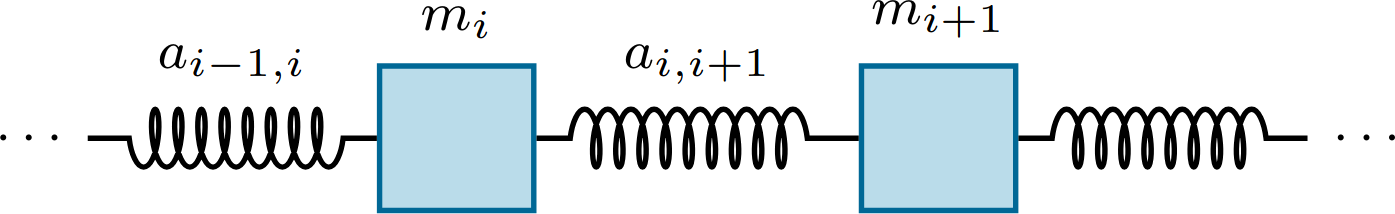
\includegraphics[width=0.5\linewidth]{./img/mass_spring_system.png}
        \end{figure}

        The elastic force $F_{e,i}(x)$ at mass $i$ is given by:
        \[
            F_{e,i}(x) = -a_{i,i-1}(x_i-x_{i-1}) - a_{i,i+1}(x_i - x_{i+1})
        \]
        Equivalently, it is possible to express the elastic force as the negative gradient of the elastic energy:
        \[
            F_{e,i}(x) = -\frac{\partial}{\partial x_i}\left( \frac{1}{2} a_{i,i-1} \Vert x_i - x_{i-1} \Vert^2 + \frac{1}{2} a_{i,i+1} \Vert x_i - x_{i+1} \Vert^2 \right)
        \]

    \item[Mass-spring system with two springs] \marginnote{Mass-spring system with two springs}
        Assume that the springs of a mass-spring system can be split with halved elastic constants.
        \begin{figure}[H]
            \centering
            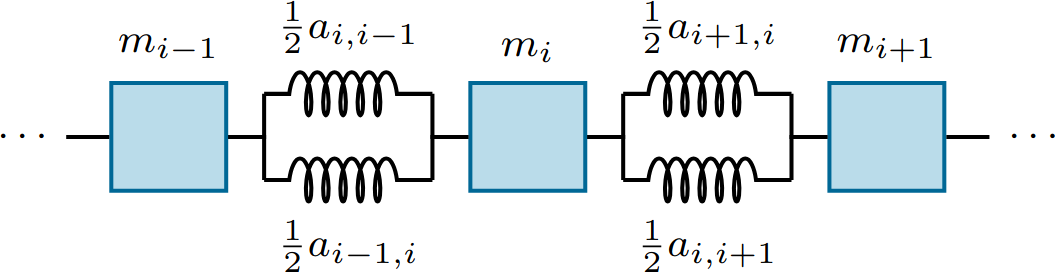
\includegraphics[width=0.5\linewidth]{./img/mass_spring_system2.png}
        \end{figure}

        Accordingly, the elastic force can be defined as:
        \[
            \small
            \begin{split}
                F_{e,i}(x) 
                &= 
                    - \frac{1}{2} a_{i,i-1}(x_i - x_{i-1}) 
                    - \frac{1}{2} a_{i-1,i}(x_i - x_{i-1}) 
                    - \frac{1}{2} a_{i,i+1}(x_i - x_{i+1}) 
                    - \frac{1}{2} a_{i+1,i}(x_i - x_{i+1}) \\
                &= 
                    - \frac{1}{2} a_{i,i-1}(x_i - x_{i-1}) 
                    + \frac{1}{2} a_{i-1,i}(x_{i-1} - x_i) 
                    - \frac{1}{2} a_{i,i+1}(x_i - x_{i+1}) 
                    + \frac{1}{2} a_{i+1,i}(x_{i+1} - x_i) \\
                &= -\frac{\partial}{\partial x_i} \left( 
                    \frac{1}{2} \frac{a_{i,i-1}}{2} \Vert x_i - x_{i-1} \Vert^2 + 
                    \frac{1}{2} \frac{a_{i-1,i}}{2} \Vert x_{i-1} - x_{i} \Vert^2 + 
                    \frac{1}{2} \frac{a_{i,i+1}}{2} \Vert x_i - x_{i+1} \Vert^2 + 
                    \frac{1}{2} \frac{a_{i+1,i}}{2} \Vert x_{i+1} - x_{i} \Vert^2 \right)
            \end{split}
        \]
        The total potential energy (i.e., sum of the function in the derivative over all masses) can be compactly defined as:
        \[
            \begin{split}
                V(x) &= \sum_{i=1}^{N} \sum_{j \in \mathcal{N}_i} \frac{1}{2} \frac{a_{i,j}}{2} \Vert x_i - x_j \Vert^2 \\
                &= \sum_{i=1}^{N} \sum_{j \in \mathcal{N}_i} V_{ij}(x_i, x_j)
            \end{split}
            \quad
            V_{i,j}(x_i, x_j) = \frac{1}{2} \frac{a_{i,j}}{2} \Vert x_i - x_j \Vert^2
        \]
        where $\mathcal{N}_i = \{ i-1, i+1 \}$.

        Then, the potential energy at mass $i$ can be written as:
        \[
            V_i(x) = \sum_{j \in \mathcal{N}_i} ( V_{i,j}(x_i, x_j) + V_{j,i}(x_j, x_i) )
        \]
            
        Finally, the elastic force at mass $i$ can be reformulated as:
        \[
            \begin{split}
                F_{e,i}(x) 
                &= - \frac{\partial}{\partial x_i} \Big( V_{i,i-1}(x_i, x_{i-1}) + V_{i-1,i}(x_{i-1}, x_i) + V_{i,i+1}(x_i, x_{i+1}) + V_{i+1,i}(x_{i+1}, x_i) \Big) \\
                &= - \frac{\partial}{\partial x_i} \left( \sum_{j \in \mathcal{N}_i} ( V_{i,j}(x_i, x_j) + V_{j,i}(x_j, x_i) ) \right) \\
                &= - \frac{\partial}{\partial x_i} V_i(x) \\
                &= - \frac{\partial}{\partial x_i} V(x)
            \end{split}
        \]

        \begin{remark}
            The system can be generalized to a graph of interconnected masses.

            \begin{figure}[H]
                \centering
                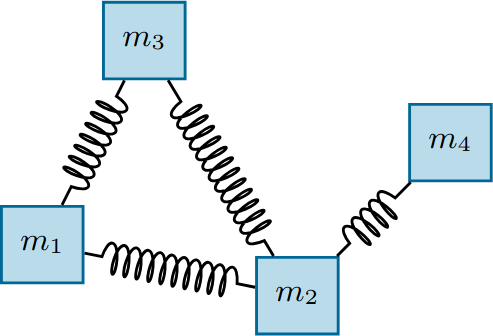
\includegraphics[width=0.3\linewidth]{./img/mass_spring_system3.png}
            \end{figure}
        \end{remark}
        
        By adding a damping coefficient (i.e., dispersion of velocity) $c=1$, the overall system dynamics can be defined as:
        \[
            \begin{split}
                \dot{x}_i &= v_i \\
                m_i \dot{v}_i &= - v_i - c\frac{\partial}{\partial x_i} V(x) = - v_i - \frac{\partial}{\partial x_i} V(x)
            \end{split}
        \]
        where $m_i$ is the mass of the $i$-th mass.

        By assuming small masses $m_i$, the following approximation can be made:
        \[
            \begin{gathered}
                \cancel{m_i \dot{v}_i} = - v_i - \frac{\partial}{\partial x_i} V(x) \Rightarrow v_i \approx -\frac{\partial}{\partial x_i} V(x) \\
                \dot{x_i} = -\frac{\partial}{\partial x_i} V(x) = F_{e,i}(x)
            \end{gathered}
        \]

        By more explicitly expanding the dynamics of the $i$-th mass, we have that:
        \[
            \begin{aligned}
                \dot{x}_i
                &= - \sum_{j \in \mathcal{N}_i} \frac{\partial}{\partial x_i} \Big( V_{i,j}(x_i, x_j) + V_{j,i}(x_j, x_i) \Big) \\
                &= - \sum_{j \in \mathcal{N}_i} \frac{\partial}{\partial x_i} \left( \frac{1}{2} \frac{a_{i,j}}{2} \Vert x_i - x_j \Vert^2 + \frac{1}{2} \frac{a_{j,i}}{2} \Vert x_j - x_i \Vert^2 \right) \\
                &= - \sum_{j \in \mathcal{N}_i} \left( \frac{1}{2} a_{i,j} (x_i - x_j) - \frac{1}{2} a_{j,i} (x_j - x_i) \right) &&& \text{\footnotesize $a_{i,j}=a_{j,i}$ ($G$ undirected)} \\
                &= - \sum_{j \in \mathcal{N}_i} a_{i,j} (x_i - x_j) &&& \text{\footnotesize i.e., Laplacian dynamics}
            \end{aligned}
        \]
        
        Therefore, the overall system follows a Laplacian dynamics and can be equivalently formulated as the gradient flow of $V$:
        \[
            \begin{split}
                \dot{\x} &= -\matr{L}\x = - \nabla V(x) \\
                \begin{bmatrix}
                    \dot{x}_1 \\ \vdots \\ \dot{x}_N
                \end{bmatrix}
                &=
                - \begin{bmatrix}
                    \frac{\partial}{\partial x_1} V(x) \\
                    \vdots
                    \\
                    \frac{\partial}{\partial x_N} V(x)
                \end{bmatrix}
            \end{split}
        \]
        And consensus is reached at a stationary point of $V(x)$.
\end{description}



\section{Formation control based on potential functions}


\begin{remark}
    The gradient flow based on the global potential function/energy can be computed in a distributed way (i.e., it depends only on neighboring states):
    \[
        \dot{x}_i(t) = - \sum_{j \in \mathcal{N}_i} \frac{\partial}{\partial x_i} \Big( V_{i,j}(x_i, x_j) + V_{j,i}(x_j, x_i) \Big)
    \]
\end{remark}


\begin{description}
    \item[Formation control] \marginnote{Formation control}
        Consider $N$ agents with states $\x_i(t) \in \mathbb{R}^d$ and communicating according to a fixed undirected graph $G$, and a set of distances $d_{ij} = d_{ji}$. The goal is to position each agent respecting the desired distances between them:
        \[
            \forall (i,j) \in E: \Vert \x_i^\text{form} - \x_j^\text{form} \Vert = d_{ij}
        \]

        To solve the problem, the potential function can be defined as:
        \[
            \begin{gathered}
                V^\text{form}(\x) = \sum_{i=1}^{N} \sum_{j \in \mathcal{N}_i} V_{ij}^\text{form}(\x_i, \x_j) \\
                V_{ij}^\text{form}(\x_i, \x_j) = \frac{1}{8} \left( \Vert \x_i - \x_j \Vert^2 - d_{ij}^2 \right)^2
            \end{gathered}
        \]
        where $\frac{1}{8}$ is used to cancel out the fraction when deriving.

        The gradient flow dynamics is then:
        \[
            \begin{split}
                \dot{\x}_i &= - \sum_{j \in \mathcal{N}_i} \frac{\partial}{\partial \x_i} \left( V_{ij}^\text{form}(\x_i, \x_j) + V_{ji}^\text{form}(\x_j, \x_i) \right) \\
                &= - \sum_{j \in \mathcal{N}_i} \left( \Vert \x_i - \x_j \Vert^2 - d_{ij}^2 \right)(\x_i - \x_j)
            \end{split}
        \]

        \begin{remark}
            Apart from the desired formation, another equilibrium of this dynamics is $x_1 = x_2 = \dots = x_N$ (i.e., a collision).
        \end{remark}

    \item[Collision avoidance potential function/Barrier function] \marginnote{Collision avoidance potential function/Barrier function}
        Function $V_{ij}^\text{ca}(\x_i, \x_j)$ such that:
        \[
            \lim_{\Vert \x_i - \x_j \Vert \rightarrow 0} V_{ij}^\text{ca}(\x_i, \x_j) = +\infty
        \]

        \begin{remark}
            A possible barrier function is:
            \[
                V_{ij}^\text{ca}(\x_i, \x_j) = - \log( \Vert \x_i - \x_j \Vert^2 - d^2 )
            \]
            where $d$ is the safety distance.
        \end{remark}

    \item[Formation control with obstacle avoidance] \marginnote{Formation control with obstacle avoidance}
        Formation control where agents avoid collisions and obstacles. The dynamics is:
        \[
            \dot{\x}_i = - \frac{\partial}{\partial \x_i} \Big( V^\text{form}(\x) + V^\text{ca}(\x) + V^\text{obs}(\x) \Big)
        \]
        where:
        \begin{itemize}
            \item $V^\text{ca}(\x) = \sum_{i=1}^N \sum_{j \in \mathcal{N}_i} V_{ij}^\text{ca}(\x_i, \x_j)$ and $V_{ij}^\text{ca}(\x_i, \x_j)$ is the barrier function to avoid collisions between agents.
            \item $V^\text{obs}(\x) = \sum_{i=1}^N V_{i}^\text{obs}(\x_i)$ and $V_{i}^\text{obs}(\x_i)$ is the barrier function to avoid collisions between an agent and an obstacle.
        \end{itemize}
\end{description}


